\documentclass[24pt,pdf,hyperref={unicode},aspectratio=169]{beamer}
\usepackage[utf8]{inputenc}
\usepackage{aiml}
\newcommand{\nothing}
{
\begin{minipage}{1cm}

\begin{tikzpicture}[x=0.5cm,y=0.5cm]
\draw[thick] (0,0)--(1,1);
\draw[thick] (0,1)--(1,0);
\end{tikzpicture}
\end{minipage}
}

\begin{document}


\section{Логика предикатов}

\begin{frame}\frametitle{Дедуктивные рассуждения}
\uncover<+->{
\begin{tabular}{l l}
 & Все страны Южной Америки -- республики \\
 & Бразилия -- страна Южной Америки\\
 \hline
$\therefore$ & Бразилия -- республика \\
\end{tabular}\\[2cm]
}
\uncover<+->{
{\large
$$
\frac{A, B}{?}
$$
}
}
\end{frame}

\begin{frame}\frametitle{Дедуктивные рассуждения}
\uncover<+->{
\begin{tabular}{l l}
 & Если страна находится в Южной Америке, то она республика \\
 & Бразилия находится в Южной Америке \\
 \hline
$\therefore$ & Бразилия -- республика \\
\end{tabular}\\[2cm]
}
\uncover<+->{
{\large
$$
\frac{A\rightarrow B, C}{?}
$$
}
}
\end{frame}

\begin{frame}\frametitle{Модель}
\begin{columns}
\column{0.5\textwidth}

\uncover<3->{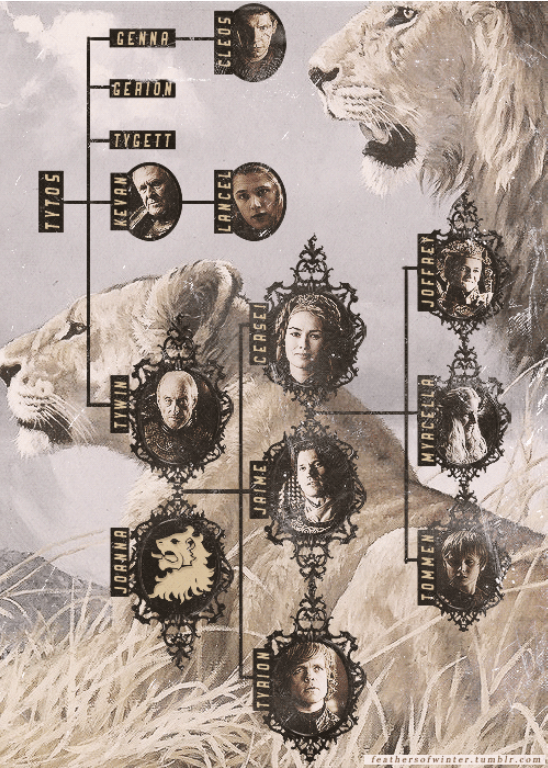
\includegraphics[scale=0.25]{tree.png}}


\column{0.5\textwidth}

\uncover<1->{$$
\mathfrak{M}=(M,P_1,\ldots,P_n)
$$}
\uncover<2->{$$
P_i:M^{k_i}\rightarrow\{0,1\}
$$}
\uncover<3->{$P(x,y)$, $C(x,y)$}
\begin{itemize}
\item<4-> $P(Tywin,Cercei)$

\item<5-> $C(Tommen,Cercei)$

\item<6-> $C(Tyrion,Cercei)$

\item<7-> $\forall x,y\ P(x,y)\rightarrow C(y,x)$

\item<8-> $\exists u,x,y,z\ C(u,x)\wedge C(u,y)\wedge C(x,z)\wedge C(y,z)$

\item<9-> $\forall x \exists y\ P(y,x)$
\end{itemize}
\end{columns}
\end{frame}

\begin{frame}\frametitle{Модель}
\uncover<+->{
\begin{center}
$\mathfrak{N}=(\mathbb{N},Eq,P,S)$

$Eq(x,y)\Leftrightarrow x=y$

$S(x,y,z) \Leftrightarrow x+y=z$

$P(x,y,z) \Leftrightarrow xy=z$
\end{center}
}
\uncover<+->{
\begin{tabular}{p{4cm} p{5cm}}
Свойство единицы & $\forall x\ P(x,1,x) \wedge P(1,x,x)$ \\
Коммутативность\newline сложения & $\forall x,y,z\ S(x,y,z)\rightarrow S(y,x,z)$\\
Отображение & $\forall x,y,z,u\ (P(x,y,u)\wedge P(x,y,v))\rightarrow Eq(u,v)$ \\
Тотальное отображение & $\forall x,y\ \exists z\ S(x,y,z)$ \\
Вычитание & $\forall x,y\ \exists z\ S(x,z,y)$ \\
\end{tabular}
}
\end{frame}

\begin{frame}\frametitle{Вывод в логике предикатов}

$$
\begin{array}{l l}
& (\forall x\ P(x))\rightarrow(\forall x\ Q(x)) \\
& (\forall x\ P(x)) \\
\hline
& A=(\forall x\ P(x)),\ B=(\forall x\ Q(x)) \\
\therefore & \forall x\ Q(x)
\end{array}
$$\\[1cm]
$$
\begin{array}{l l}
& \forall x\ P(x)\rightarrow Q(x) \\
& P(a) \\
\hline
\therefore & Q(a)
\end{array}
$$
\end{frame}

\section{Предваренная нормальная форма}

\begin{frame}\frametitle{Предваренная нормальная форма}
\begin{enumerate}
\item<1-> Оставить только $\wedge$, $\vee$, $\neg$
\item<2-> Протаскивание отрицаний: законы де Моргана и

$$
\neg(\forall x\ P(x))\Leftrightarrow \exists x\ \neg P(x)
$$
$$
\neg(\exists x\ P(x))\Leftrightarrow \forall x\ \neg P(x)
$$
\item<3-> { Вытаскивание кванторов }

\begin{center}

\uncover<4->{$
(\forall x\ P(x))\wedge(\forall x\ Q(x))\Leftrightarrow \forall x\ (P(x)\wedge Q(x))
$}

\only<5>{$
(\exists x\ P(x))\wedge(\exists x\ Q(x))\Leftrightarrow \exists x\ (P(x)\wedge Q(x) )
$}
\uncover<6->{$
(\exists x\ P(x))\wedge(\exists x\ Q(x))\Leftrightarrow \exists x\exists y\ (P(x)\wedge Q(y))
$}


\uncover<7->{$
(\exists x\ P(x))\vee(\exists x\ Q(x))\Leftrightarrow \exists x\ (P(x)\vee Q(x))
$}


\uncover<8->{$
(\forall x\ P(x))\vee(\forall x\ Q(x))\Leftrightarrow \forall x\forall y\ (P(x)\vee Q(x))
$}
\end{center}
\item<9-> Результат: предваренная нормальная форма

$$
\forall x_1 \forall x_2 \exists x_3 \forall x_4\ F
$$
\end{enumerate}

\end{frame}


\begin{frame}\frametitle{Предваренная нормальная форма}

\begin{itemize}
\item<+-> $(\forall x\ P(x))\oplus (\exists x\ Q(x))$
\item<+-> $\left[\overline{(\forall x\ P(x))}\wedge(\exists x\ Q(x))\right] \bigvee \left[(\forall x\ P(x))\wedge\overline{(\exists x\ Q(x)})\right]$
\item<+-> $\left[(\exists x\ \overline{P(x)})\wedge(\exists x\ Q(x))\right] \bigvee \left[(\forall x\ P(x))\wedge\overline{(\exists x\ Q(x)})\right]$
\item<+-> $\left[(\exists x\ \overline{P(x)})\wedge(\exists x\ Q(x))\right] \bigvee \left[(\forall x\ P(x))\wedge(\forall x\ \overline{Q(x)})\right]$
\item<+-> $\left[\exists x \exists y\ \overline{P(x)}\wedge Q(y)\right] \bigvee \left[(\forall x\ P(x))\wedge(\forall x\ \overline{Q(x)})\right]$
\item<+-> $\left[\exists x \exists y\ \overline{P(x)}\wedge Q(y)\right] \bigvee \left[\forall x\ P(x)\wedge\overline{Q(x)}\right]$
\item<+-> $\left[\exists x \exists y\ \overline{P(x)}\wedge Q(y)\right] \bigvee \left[\forall z\ P(z)\wedge\overline{Q(z)}\right]$
\item<+-> $\exists x \exists y \forall z \left[ (\overline{P(x)}\wedge Q(y)) \vee (P(z)\wedge\overline{Q(z)})\right]$
\end{itemize}
\end{frame}
\begin{frame}\frametitle{Предваренная нормальная форма}
\begin{itemize}
\item<+-> $\exists x \exists y \forall z \left[ (\overline{P(x)}\wedge Q(y)) \vee (P(z)\wedge\overline{Q(z)})\right]$

\item<+-> $\exists x \exists y \forall z \left[ (\overline{P(x)}\vee P(z))\wedge (\overline{P(x)}\vee \overline{Q(z)}) \wedge \right.$

\hspace{3cm} $ \left. \wedge (Q(y) \vee P(z)) \wedge (Q(y) \vee \overline{Q(z)}) \right] $

\item<+-> $\exists x \exists y \forall z \left[ (\overline{P(x)}\vee \overline{Q(z)}) \wedge (Q(y) \vee P(z))  \right]$

\end{itemize}
\end{frame}


\section{Сколемовская нормальная форма}

\begin{frame}\frametitle{Сколемовская нормальная форма}
\begin{itemize}
\item<+-> $\exists t \forall u \exists v\forall x \forall y \exists z\ P(t,u,v)\vee P(x,y,z)$
\item<+-> $\forall u \exists v\forall x \forall y \exists z\ P(a,u,v)\vee P(x,y,z)$ 
\item<+-> $\forall u \forall x \forall y \exists z\ P(a,u,f(u))\vee P(x,y,z)$ 
\item<+-> $\forall u \forall x \forall y \ P(a,u,f(u))\vee P(x,y,g(u,x,y))$ 
\item<+-> $P(a,u,f(u))\vee P(x,y,g(u,x,y))$ 
\item<+-> $P(a,u,f(u)),\ P(x,y,g(u,x,y))$ 
\end{itemize}
\end{frame}

\section{Правило резолюций. Унификация}

\begin{frame}\frametitle{Правило резолюций в логике предикатов}
$$
\begin{array}{l l}
\uncover<+->{
 & \neg P(x) \vee Q(x) \\
 & P(a) \\
 \hline
}
\uncover<+->{
 & x:=a \\
 & \neg P(a) \vee Q(a) \\
 & P(a) \\
 \hline
}
\uncover<+->{
\therefore & Q(a) \\
}
\end{array}
$$
\end{frame}

\begin{frame}\frametitle{Удачные и неудачные унификации}

$$
\uncover<+->{
\begin{array}{l}
P(f(x))\vee Q(x) \\
\neg P(f(a))
\end{array}
}
\uncover<+->{
\Rightarrow
\begin{array}{l}
x:=a\\
Q(a)
\end{array}
}
$$

$$
\uncover<+->{
\begin{array}{l}
P(x,a))\vee Q(x) \\
\neg P(b,c)
\end{array}
}
\uncover<+->{
\Rightarrow
\nothing
}
$$

$$
\uncover<+->{
\begin{array}{l}
P(x,a)\vee Q(x) \\
\neg P(b,x)
\end{array}
}
\uncover<+->{
\Rightarrow
\begin{array}{l}
P(x,a)\vee Q(x) \\
\neg P(b,y)
\end{array}
}
\uncover<+->{
\Rightarrow
\begin{array}{l}
x:=b\\
y:=a\\
Q(b)\\
\end{array}
}
$$

$$
\uncover<+->{
\begin{array}{l}
P(a,y)\vee Q(g(y)) \\
\neg P(x,f(x))
\end{array}
}
\uncover<+->{
\Rightarrow
\begin{array}{l}
x:=a\\
y:=f(a)\\
Q(g(f(b)))\\
\end{array}
}
$$
\end{frame}

\section{Доказательство теорем}


\begin{frame}\frametitle{Аксиомы теории групп}
$\mathcal{G}=(\mathbb{G},\cdot)$

\begin{itemize}
\item<+-> $\forall x,y,z,u\ (x\cdot y=z) \wedge (x\cdot y=u)\rightarrow (z=u)$

\item<+-> $\forall x,y,z\ (x\cdot (y\cdot z))=((x\cdot y)\cdot z) $

\item<+-> $\exists e\forall x\ (x\cdot e)=(e\cdot x)=x$

\item<+-> $\forall x\exists y\ (x\cdot y)=(y \cdot x)=e$
\end{itemize}
\uncover<+->{Доказать единственность единицы:}

\begin{itemize}
\item<+-> $\forall i\ \left[\forall x\ (x\cdot i)=(i\cdot x)=x\right]\rightarrow (e=i)$
\end{itemize}

\uncover<+->{Доказательство}
\begin{itemize}
\item<+-> $(i\cdot e)=i$
\item<+-> $(i\cdot e)=e$
\item<+-> $\therefore e=i$
\end{itemize}
\end{frame}


\begin{frame}\frametitle{Формализация аксиом}
$$
\mathfrak{G}=(\mathbb{G},Eq,G)
$$
$$Eq(x,y)\Leftrightarrow x=y$$
$$G(x,y,z)\Leftrightarrow x\cdot y=z$$

$$
\forall x,y,z,u\ (x\cdot y=z) \wedge (x\cdot y=u)\rightarrow (z=u)
$$
\begin{itemize}
\item<+-> $\forall x \forall y \forall z \forall u\ G(x,y,z) \wedge G(x,y,u)\rightarrow Eq(z,u)$
\item<+-> $\forall x \forall y \forall z \forall u\ \overline{G(x,y,z) \wedge G(x,y,u)}\vee Eq(z,u)$
\item<+-> $\forall x \forall y \forall z \forall u\ \neg G(x,y,z) \vee \neg G(x,y,u)\vee Eq(z,u)$
\item<+-> $\neg G(x,y,z) \vee \neg G(x,y,u)\vee Eq(z,u)$
\end{itemize}
\end{frame}

\begin{frame}\frametitle{Формализация аксиом}
$$
\exists e\forall x\ (x\cdot e)=(e\cdot x)=x
$$
\begin{itemize}
\item<+-> $\exists e\forall x\ G(x,e,x)\wedge G(e,x,x)$
\item<+-> $G(x,e,x)\wedge G(e,x,x)$
\item<+-> $G(t,e,t),\ G(e,t,t)$
\end{itemize}
\end{frame}

\begin{frame}\frametitle{Формализация теоремы}
$$
\forall i\ \left[\forall x\ (x\cdot i)=(i\cdot x)=x\right]\rightarrow (e=i)
$$
\begin{itemize}
\item<+-> $\forall i\ \left[\forall x\ G(x,i,x)\wedge G(i,x,x) \right]\rightarrow Eq(e,i)$
\item<+-> $\overline{\forall i\ \left[\forall x\ G(x,i,x)\wedge G(i,x,x) \right]\rightarrow Eq(e,i)}$
\item<+-> $\overline{\forall i\ \overline{\left[\forall x\ G(x,i,x)\wedge G(i,x,x) \right]}\vee Eq(e,i)}$
\item<+-> $\exists i\ \overline{\overline{\left[\forall x\ G(x,i,x)\wedge G(i,x,x) \right]}\vee Eq(e,i)}$
\item<+-> $\exists i\ \overline{\overline{\left[\forall x\ G(x,i,x)\wedge G(i,x,x) \right]}}\wedge \neg Eq(e,i)$
\item<+-> $\exists i\ \left[\forall x\ G(x,i,x)\wedge G(i,x,x) \right]\wedge \neg Eq(e,i)$
\item<+-> $\exists i\forall x\  G(x,i,x)\wedge G(i,x,x) \neg Eq(e,i)$
\item<+-> $G(x,i,x)\wedge G(i,x,x) \wedge \neg Eq(e,i)$
\item<+-> $G(s,i,s),\ G(i,s,s),\ \neg Eq(e,i)$
\end{itemize}
\end{frame}

\begin{frame}\frametitle{Доказательство теоремы}

\uncover<+->{}

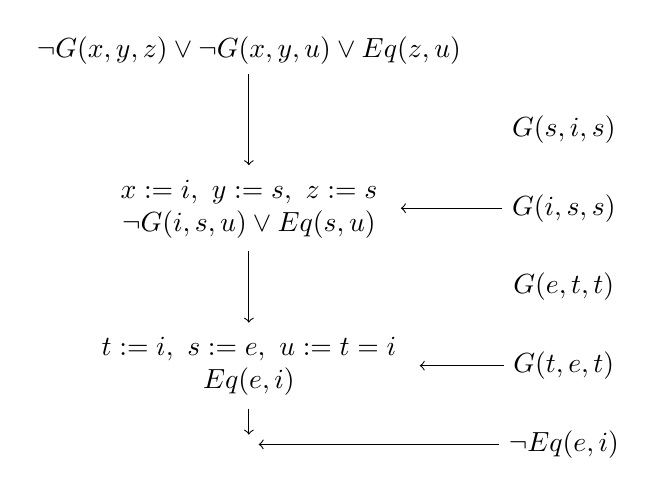
\begin{tikzpicture}

\node (eq) at (0,5) {$\neg G(x,y,z) \vee \neg G(x,y,u)\vee Eq(z,u)$};
\node (i1) at (4,4) {$G(s,i,s)$};
\node (i2) at (4,3) {$G(i,s,s)$};
\node (e2) at (4,2) {$G(e,t,t)$};
\node (e1) at (4,1) {$G(t,e,t)$};
\node (neq) at (4,0) {$\neg Eq(e,i)$};

\uncover<+->{
\node(s1) at (0,3) {$\begin{array}{c}x:=i,\ y:=s,\ z:=s\\ \neg G(i,s,u)\vee Eq(s,u)\end{array}$};
\path (eq) edge[->] (s1);
\path (i2) edge[->] (s1);
}

\uncover<+->{
\node(s2) at (0,1) {$\begin{array}{c}t:=i,\ s:=e,\ u:=t=i\\  Eq(e,i)\end{array}$};
\path (e1) edge[->] (s2);
\path (s1) edge[->] (s2);
}

\uncover<+->{
\node(s3) at (0,0) {$\square$};
\path (s2) edge[->] (s3);
\path (neq) edge[->] (s3);
}
\end{tikzpicture}
\end{frame}

\section{Поиск теорем}

\begin{frame}\frametitle{Поиск теоремы}
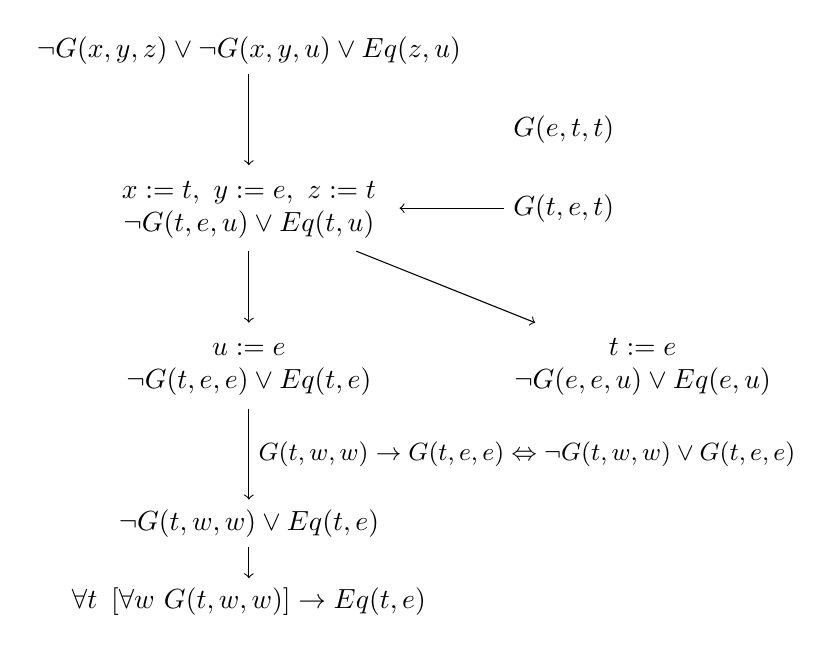
\begin{tikzpicture}
\node (eq) at (0,5) {$\neg G(x,y,z) \vee \neg G(x,y,u)\vee Eq(z,u)$};
\node (e2) at (4,4) {$G(e,t,t)$};
\node (e1) at (4,3) {$G(t,e,t)$};


\uncover<2->{
\node(s1) at (0,3) {$\begin{array}{c}x:=t,\ y:=e,\ z:=t\\ \neg G(t,e,u)\vee Eq(t,u)\end{array}$};
\path (eq) edge[->] (s1);
\path (e1) edge[->] (s1);
}

\uncover<3->{
\node(s2) at (0,1) {$\begin{array}{c}u:=e \\ \neg G(t,e,e)\vee Eq(t,e)\end{array}$};
\path (s1) edge[->] (s2);
}

\only<4>{
\node(s3) at (5,1) {$\begin{array}{c}t:=e \\ \neg G(e,e,u)\vee Eq(e,u)\end{array}$};
\path (s1) edge[->] (s3);
}

\uncover<5->{
\node(s3) at (0,-1) {$\neg G(t,w,w)\vee Eq(t,e)$};
\path (s2) edge[->] node[right]{\small $G(t,w,w)\rightarrow G(t,e,e)\Leftrightarrow \neg G(t,w,w)\vee G(t,e,e)$} (s3);
}

\uncover<6->{
\node(s4) at (0,-2) {$\forall t\ \left[\forall w\ G(t,w,w)\right]\rightarrow Eq(t,e)$};
\path (s3) edge[->] (s4);
}


\end{tikzpicture}
\end{frame}

\begin{frame}\frametitle{Зацикливание метода резолюций}
\uncover<+->{}
$$
\begin{array}{l}
P(a) \\
\neg P(x) \vee P(f(x))\\
\hline \\
\end{array}
$$
\uncover<+->{$$
\begin{array}{l}
P(f(a)) \\
\neg P(x) \vee P(f(x))\\
\hline \\
\end{array}
$$}
\uncover<+->{$$
\begin{array}{l}
P(f(f(a))) \\
\neg P(x) \vee P(f(x))\\
\hline
\ldots \\
\end{array}
$$}
\end{frame}

\begin{frame}\frametitle{Robbin's conjecture}
$$
\begin{array}{l l}
& (A\vee B)\vee C = A \vee (B\vee C) \\
& A\vee B=B\vee A \\
& \neg( \neg(A\vee B) \vee \neg(A\vee \neg B) ) = A\\
\hline 
\therefore & \neg \neg A=A
\end{array}
$$
\end{frame}

\section{Логическое программирование}


\newcommand{\myrect}[5] 
{
\draw[thick] (#1,#2) rectangle ($(#1+#3,#2+#4)$); 
\node at ($(#1,#2)+(#3 /2,#4 /2)$) {#5};
}
\usetikzlibrary{calc}

\begin{frame}
\begin{columns}
\column{0.5\textwidth}

\uncover<1->{
\begin{tikzpicture}[x=0.7cm, y=0.7cm]
\myrect{0}{0}{6.5}{1}{Table}
\myrect{0.5}{1}{1}{1}{A}
\myrect{2}{1}{1.5}{1.5}{B}
\myrect{4}{1}{2}{2}{C}
\end{tikzpicture}
}

{\small
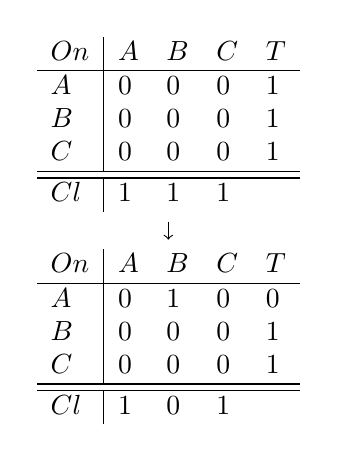
\begin{tikzpicture}[x=1cm,y=-2.7cm]
\uncover<3->{
\node(a+b+c) at (0,0) {$
\begin{array}{l|l l l l}
On & A & B & C & T \\
\hline
A  & 0 & 0 & 0 & 1 \\
B  & 0 & 0 & 0 & 1 \\
C  & 0 & 0 & 0 & 1 \\
\hline\hline 
Cl & 1 & 1 & 1 & \\
\end{array}$};
}

\uncover<4->{
\node(ab+c) at (0,1) {$
\begin{array}{l|l l l l}
On & A & B & C & T \\
\hline
A  & 0 & 1 & 0 & 0 \\
B  & 0 & 0 & 0 & 1 \\
C  & 0 & 0 & 0 & 1 \\
\hline\hline 
Cl & 1 & 0 & 1 & \\
\end{array}$};

\path (a+b+c) edge[->] (ab+c);
}


\end{tikzpicture}
}


\column{0.5\textwidth}

\uncover<2->{
Действие:

\begin{itemize}
\item $ Move(what,from,to)$
\end{itemize}

Требования:


\begin{itemize}
\item $On(what,from)$
\item $Cl(to) \vee (to=Table)$
\item $Cl(what)$
\end{itemize}

Результат:

\begin{itemize}
\item $On(what,to)$
\item $\neg Cl(to)$
\item $\neg On(what,from)$
\item $Cl(from)$
\end{itemize}
}

\end{columns}
\end{frame}

\begin{frame}
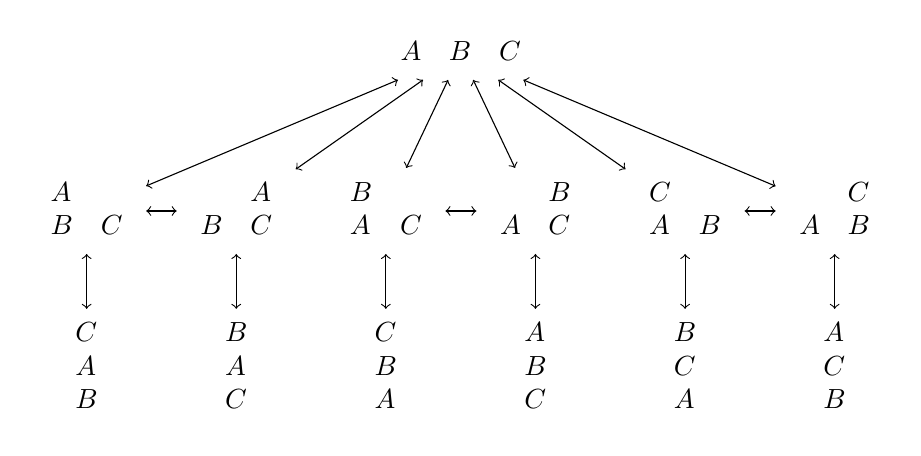
\begin{tikzpicture}[x=1.9cm, y=-2cm]

\uncover<1->{
\node (a+b+c) at (2.5,0) {$\begin{array}{l l l} A & B & C \end{array}$};
}

\uncover<2->{
\node(ab+c) at (0,1) {$\begin{array}{l l} A \\ B & C \end{array}$};
\path (a+b+c) edge[<->] (ab+c);
}

\uncover<3->{
\node(ac+b) at (1,1) {$\begin{array}{l l} & A \\ B & C \end{array}$};
\node(ba+c) at (2,1) {$\begin{array}{l l} B \\ A & C \end{array}$};
\node(bc+a) at (3,1) {$\begin{array}{l l} & B \\ A & C \end{array}$};
\node(ca+b) at (4,1) {$\begin{array}{l l} C \\ A & B \end{array}$};
\node(cb+a) at (5,1) {$\begin{array}{l l} & C \\ A & B \end{array}$};

\path (a+b+c) edge[<->] (ac+b);
\path (a+b+c) edge[<->] (ba+c);
\path (a+b+c) edge[<->] (bc+a);
\path (a+b+c) edge[<->] (ca+b);
\path (a+b+c) edge[<->] (cb+a);
}

\uncover<4->{
\path (ab+c) edge[<->] (ac+b);
\path (ba+c) edge[<->] (bc+a);
\path (ca+b) edge[<->] (cb+a);
}

\uncover<5->{
\node(cab) at (0,2) {$\begin{array}{l} C \\ A \\ B \end{array}$};
\node(bac) at (1,2) {$\begin{array}{l} B \\ A \\ C \end{array}$};
\node(cba) at (2,2) {$\begin{array}{l} C \\ B \\ A \end{array}$};
\node(abc) at (3,2) {$\begin{array}{l} A \\ B \\ C \end{array}$};
\node(bca) at (4,2) {$\begin{array}{l} B \\ C \\ A \end{array}$};
\node(acb) at (5,2) {$\begin{array}{l} A \\ C \\ B \end{array}$};

\path (ab+c) edge[<->] (cab);
\path (ac+b) edge[<->] (bac);
\path (ba+c) edge[<->] (cba);
\path (bc+a) edge[<->] (abc);
\path (ca+b) edge[<->] (bca);
\path (cb+a) edge[<->] (acb);
}

\end{tikzpicture}
\end{frame}

\begin{frame}
\begin{center}
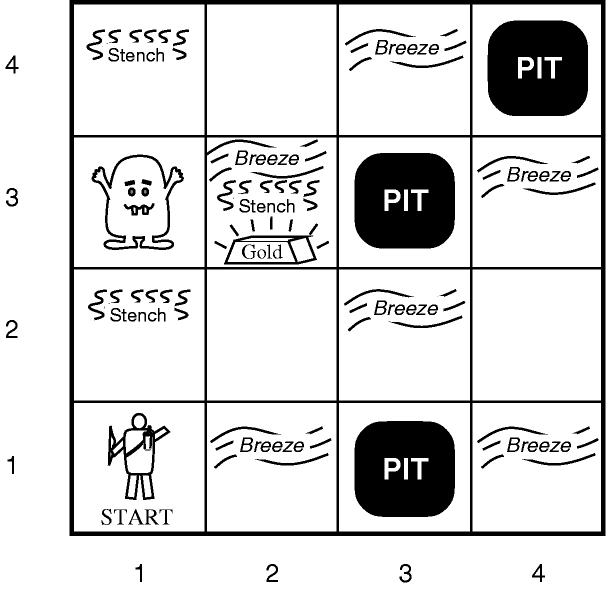
\includegraphics[width=0.65\textwidth]{wumpus.png}
\end{center}
\end{frame}


\end{document}
